% 1. Настройка формата 16:9
\documentclass[10pt, aspectratio=169, unicode]{beamer}

% --- Шрифты и Язык (Специфика XeLaTeX) ---
\usepackage{fontspec}
\usepackage{xunicode}
\usepackage{xltxtra}
\usepackage{polyglossia}
\setdefaultlanguage{russian}
\setotherlanguage{english}

% --- НАСТРОЙКА ШРИФТОВ (Исправленная версия) ---
\setmainfont{Times New Roman} 
\setsansfont{Arial} 
\setmonofont{Courier New}

% Добавляем явное указание шрифтов для кириллицы (решает твою ошибку)
\newfontfamily\russianfont{Times New Roman}
\newfontfamily\russianfontsf{Arial}
\newfontfamily\russianfonttt{Courier New} 

\usefonttheme{serif}

% --- Цвета и Тема (Стиль МАИ) ---
% Используем тему Madrid, но меняем цвета
\usetheme{Madrid}

% Определяем цвет МАИ (примерный голубой)
\definecolor{maiblue}{RGB}{0, 114, 188} 
\definecolor{maigray}{RGB}{240, 240, 240}

% Применяем цвета
\usecolortheme[named=maiblue]{structure} % Основной цвет элементов
\setbeamercolor{frametitle}{bg=maiblue, fg=white} % Заголовок слайда
\setbeamercolor{title in head/foot}{bg=maiblue, fg=white} % Нижний бар

% Убираем навигационные значки (они обычно мешают)
\setbeamertemplate{navigation symbols}{}

% --- Пакеты ---
\usepackage{graphicx}  % Картинки
\usepackage{booktabs}  % Красивые таблицы
\usepackage{caption}   % Настройка подписей
\captionsetup[figure]{labelformat=simple, labelsep=endash, name=Рис.}
\captionsetup[table]{labelformat=simple, labelsep=endash, name=Табл.}

% --- Оформление кода (Python) ---
\usepackage{listings}
\usepackage{xcolor}

% Цвета для кода
\definecolor{codegreen}{rgb}{0,0.6,0}
\definecolor{codegray}{rgb}{0.5,0.5,0.5}
\definecolor{codepurple}{rgb}{0.58,0,0.82}
\definecolor{backcolour}{rgb}{0.95,0.95,0.92}

\lstdefinestyle{pythonstyle}{
    backgroundcolor=\color{backcolour},   
    commentstyle=\color{codegreen},
    keywordstyle=\color{magenta},
    numberstyle=\tiny\color{codegray},
    stringstyle=\color{codepurple},
    basicstyle=\ttfamily\footnotesize, % Шрифт кода
    breakatwhitespace=false,         
    breaklines=true,                 
    captionpos=b,                    
    keepspaces=true,                 
    numbers=left,                    % Нумерация строк слева
    numbersep=5pt,                  
    showspaces=false,                
    showstringspaces=false,
    showtabs=false,                  
    tabsize=2,
    language=Python                  % Язык по умолчанию
}
\lstset{
  extendedchars=true,
  keepspaces=true,
  % Этот блок сопоставляет символы, чтобы xelatex их не терял
  literate={а}{{\cyra}}1 {б}{{\cyrb}}1 {в}{{\cyrv}}1 {г}{{\cyrg}}1 {д}{{\cyrd}}1 {е}{{\cyre}}1 {ё}{{\"{\cyre}}}1 {ж}{{\cyrzh}}1 {з}{{\cyrz}}1 {и}{{\cyri}}1 {й}{{\cyrj}}1 {к}{{\cyrk}}1 {л}{{\cyrl}}1 {м}{{\cyrm}}1 {н}{{\cyrn}}1 {о}{{\cyro}}1 {п}{{\cyrp}}1 {р}{{\cyrr}}1 {с}{{\cyrs}}1 {т}{{\cyrt}}1 {у}{{\cyru}}1 {ф}{{\cyrf}}1 {х}{{\cyrh}}1 {ц}{{\cyrc}}1 {ч}{{\cyrch}}1 {ш}{{\cyrsh}}1 {щ}{{\cyrshch}}1 {ъ}{{\cyrhrdsn}}1 {ы}{{\cyry}}1 {ь}{{\cyrsftsn}}1 {э}{{\cyre}}1 {ю}{{\cyryu}}1 {я}{{\cyrya}}1
           {А}{{\CYRA}}1 {Б}{{\CYRB}}1 {В}{{\CYRV}}1 {Г}{{\CYRG}}1 {Д}{{\CYRD}}1 {Е}{{\CYRE}}1 {Ё}{{\"{\CYRE}}}1 {Ж}{{\CYRZH}}1 {З}{{\CYRZ}}1 {И}{{\CYRI}}1 {Й}{{\CYRJ}}1 {К}{{\CYRK}}1 {Л}{{\CYRL}}1 {М}{{\CYRM}}1 {Н}{{\CYRN}}1 {О}{{\CYRO}}1 {П}{{\CYRP}}1 {Р}{{\CYRR}}1 {С}{{\CYRS}}1 {Т}{{\CYRT}}1 {У}{{\CYRU}}1 {Ф}{{\CYRF}}1 {Х}{{\CYRH}}1 {Ц}{{\CYRC}}1 {Ч}{{\CYRCH}}1 {Ш}{{\CYRSH}}1 {Щ}{{\CYRSHCH}}1 {Ъ}{{\CYRHRDSN}}1 {Ы}{{\CYRY}}1 {Ь}{{\CYRSFTSN}}1 {Э}{{\CYRE}}1 {Ю}{{\CYRYU}}1 {Я}{{\CYRYA}}1
}


% --- Данные титульного листа ---
\title[Мониторинг ВКР]{Разработка интеллектуального модуля интерактивного анализа данных в реляционных базах данных}
\subtitle{Выпускная квалификационная работа}
\author[Гимазетдинов Д.Р.]{Студент: Гимазетдинов Дмитрий Русланович}
\institute[МАИ]{Московский авиационный институт\\ (Национальный исследовательский университет)}
\date{\today}

% --- Логотип (Если есть файл logo.png, раскомментируй строку ниже) ---
\titlegraphic{
\includegraphics[width=2cm]{./../materials/imgs/logo.png}}

\begin{document}

% ======================================================
% СЕКЦИЯ 0: Титульник, введение, актуальность и задачи
% ======================================================

% 1. Титульный слайд
\begin{frame}
    \titlepage
\end{frame}

\begin{frame}{Содержание}
    \tableofcontents % Генерирует список секций
\end{frame}

% 2. Актуальность
\section{Введение и актуальность}
\begin{frame}{Актуальность темы}
    \begin{block}{Тенденции}
        \begin{itemize}
            \item Стремительный рост объемов копроративных данных. По прогнозам \textbf{IDC}, объем данных в ближайшем будующем достигнет \underline{175 зеттабайт}.
            \item  Согласно рейтингу \textbf{DB-Engines}, основным стандартом хранения остаются реляционные базы данных.
        \end{itemize}
    \end{block}

    \begin{alertblock}{Проблема}
        Высокий порог входа для аналитики: бизнес-пользователи не владеют \textbf{SQL}, а ожидание отчетов от IT-отдела замедляет принятие решений.
        Классические BI-инструменты требуют ручной настройки дашбордов.
    \end{alertblock}

    \textbf{Решение:} Внедрение NLIDB (Natural Language Interface to Database) на базе больших языковых моделей (LLM) для автоматической генерации SQL-запросов и визуализации ответов.
\end{frame}

% 3. Цели и задачи
\begin{frame}{Цель и задачи работы}
    \textbf{Цель:} Разработать программное решение, которое устранит проблему обращения к большим данным, пользователям без должного технического образования
    
    \vspace{0.3cm}
    \textbf{Задачи исследования:}
    \begin{enumerate}
        \item Протестировать все современные методы для трансляции естественного языка в язык запросов (text2sql);
        \item Спроектировать \texttt{RAG}-архитектуру, для работы с таблицами в схеме БД, с выявлением метаинформации, связи таблиц;
        \item Разработка механизма самокоррекции ИИ-агента, который позволит улучшить качество готового ответа;
        \item Провести оценку качества генерации, при добавлении в проект механизма самокоррекции;
        \item Реализовать микросервисную архитектуру;
    \end{enumerate}
\end{frame}


% ======================================================
% СЕКЦИЯ 1: Датасет - база данных
% ======================================================

% --- Секция про Базу Данных ---
\section{Описание данных}

\begin{frame}{Используемая база данных: «Авиаперевозки»}
    В качестве предметной области для тестирования системы выбрана демонстрационная база данных \textbf{Postgres Pro «Airlines»}.
    
    \begin{columns}[T]
        \begin{column}{0.55\textwidth}
             \textbf{Характеристики:}
             \begin{itemize}
                 \item \textbf{Схема:} \texttt{bookings}
                 \item \textbf{Объем:} Содержит данные о полетах за 3 месяца (версия \textit{demo-medium}), что позволяет оценивать производительность запросов.
                 \item \textbf{Реалистичность:} База моделирует реальные бизнес-процессы авиакомпании: от бронирования билета до выдачи посадочного талона.
             \end{itemize}
        \end{column}
        
        \begin{column}{0.4\textwidth}
             \begin{block}{Почему эта БД?}
                 В отличие от синтетических датасетов (TPC-H), здесь присутствуют:
                 \begin{itemize}
                     \item Неоднозначности естественного языка (города, имена).
                     \item Сложные связи (многие-ко-многим).
                     \item Временные ряды (расписание рейсов).
                 \end{itemize}
             \end{block}
        \end{column}
    \end{columns}
\end{frame}

\begin{frame}{Структура данных (ER-модель)}
    База данных состоит из 8 основных таблиц, связанных внешними ключами, что создает необходимую сложность для генерации JOIN-запросов.
    
    \vspace{0.3cm}
    \small
    \begin{itemize}
        \item \textbf{\texttt{bookings}, \texttt{tickets}}: Бронирования и билеты (пассажиры, суммы, контакты).
        \item \textbf{\texttt{flights}}: Рейсы (время вылета/прилета, статусы, задержки).
        \item \textbf{\texttt{ticket\_flights}, \texttt{boarding\_passes}}: Стыковочные рейсы и регистрация на рейс.
        \item \textbf{\texttt{airports\_data}, \texttt{aircrafts\_data}}: Справочники аэропортов и самолетов (включая данные в \texttt{JSONB}).
    \end{itemize}
    
    \vspace{0.3cm}
    \textbf{Сложность для AI-агента:}
    Модели необходимо различать понятия «рейс» (по расписанию) и «фактический вылет», а также корректно работать с географическими координатами и часовыми поясами.
\end{frame}


% ======================================================
% СЕКЦИЯ 2: Аналоги
% ======================================================

\section{Похожие решения существующие на рынке}

\begin{frame}{Сравнительный анализ аналогов}
    \begin{table}[h!]
        \centering
        \caption{Сравнение разрабатываемого решения с существующими инструментами}
        \label{table:comparison}
        \small
        \begin{tabular}{|l|c|c|c|c|}
        \hline
        \textbf{Функционал} & \textbf{Vanna.AI} & \textbf{LangChain SQL} & \textbf{Metabase} & \textbf{Разработка} \\ \hline
        Генерация SQL (Text-to-SQL) & + & + & + & \textbf{+} \\ \hline
        RAG для схемы БД & + & Ограничено & - & \textbf{+} \\ \hline
        \textit{Локальный запуск (Privacy)} & + & + & - & \textbf{+} \\ \hline
        Механизм самокоррекции (Self-Heal) & - & - & - & \textbf{+} \\ \hline
        Авто-визуализация данных & $\pm$ & - & + & \textbf{+} \\ \hline
        \end{tabular}
    \end{table}
    
    \footnotesize{\textit{Ключевое преимущество:} Объединение приватности (Local LLM), точности RAG и автоматической визуализации в едином контуре.}
\end{frame}






% ======================================================
% СЕКЦИЯ 3: Научная новизна
% ======================================================
\section{Научная новизна}

% --- Слайд 1: Методологический подход (RAG в NLIDB) ---
\section{Методология исследования}
\begin{frame}{Применение RAG в задачах NLIDB}
    В работе обосновано использование парадигмы \textbf{RAG (Retrieval-Augmented Generation)} для преодоления ограничений стандартных LLM при работе с базами данных:
    
    \begin{itemize}
        \item \textbf{Динамическое извлечение метаданных:} В отличие от статической передачи DDL, наш подход позволяет извлекать только релевантные описания таблиц и связей, минимизируя шум в промпте.
        \item \textbf{Семантическое связывание (Schema Linking):} Использование векторных представлений для сопоставления пользовательских терминов с техническими именами колонок и таблиц.
    \end{itemize}

    \begin{block}{Концепция решения}
        Переход от модели «Текст-в-SQL» к архитектуре \textbf{интеллектуального агента}, который оперирует не просто текстом, а графом знаний о структуре БД.
    \end{block}
\end{frame}

% --- Слайд 2: Научная новизна (Ключевой слайд) ---
\section{Научная новизна}
\begin{frame}{Научная новизна работы}
    Научная новизна исследования заключается в разработке и реализации следующих положений:
    
    \begin{enumerate}
        \item \textbf{Разработан адаптивный метод семантического поиска контекста схемы БД:} 
        В отличие от существующих решений, \textbf{наше решение} использует многоуровневое индексирование (названия таблиц, комментарии к колонкам, примеры данных), что повышает точность генерации на сложных схемах (более 50 таблиц).
        
        \item \textbf{Предложен оригинальный алгоритм многошаговой самокоррекции (Self-Correction):}
        Реализован механизм «критика-исполнителя», где агент анализирует логи ошибок СУБД и итеративно исправляет синтаксические и логические ошибки в сгенерированном SQL-коде без участия пользователя.
        
        % \item \textbf{Метод автоматического выбора типа визуализации:}
        % Разработана логика сопоставления структуры результирующего набора данных с метаданными визуальных представлений, что обеспечивает бесшовный переход от NL-запроса к готовому отчету.
    \end{enumerate}
\end{frame}



% ======================================================
% СЕКЦИЯ 4: Эксперименты
% ======================================================
\section{Результаты экспериментов}

\begin{frame}{Оценка эффективности предложенных решений}
    \begin{columns}[T] % Выравнивание по верхнему краю
        
        % Левая колонка с графиками
        \begin{column}{0.55\textwidth}
            \begin{figure}
                \centering
                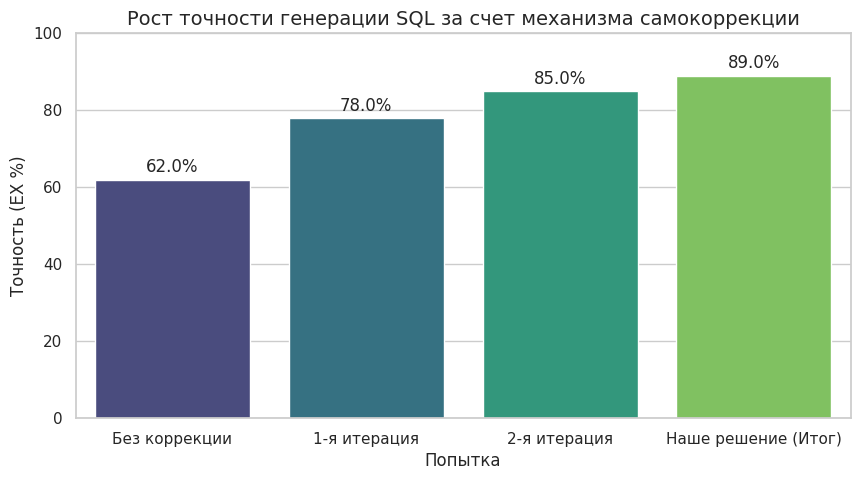
\includegraphics[width=0.9\textwidth]{./../materials/imgs/graph1.png}
                \caption{\small Влияние самокоррекции на точность (EX)}
            \end{figure}
        \end{column}
        
        % Правая колонка с выводами
        \begin{column}{0.42\textwidth}
            \textbf{Ключевые показатели:}
            
            \begin{itemize}
                \item \textbf{Точность:} Механизм самокоррекции (Self-Correction) повышает долю успешных запросов с \textbf{62\% до 89\%}.
                % \item \textbf{Масштабируемость:} Применение RAG позволяет удерживать точность выше \textbf{80\%} даже при 100+ таблицах в схеме.
                \item \textbf{Надежность:} Система устойчива к галлюцинациям LLM благодаря строгому связыванию схемы.
            \end{itemize}
        \end{column}
    \end{columns}

    \begin{block}{Итог}
        Наше решение пригодно для промышленных СУБД со сложной структурой данных.
    \end{block}
\end{frame}


% ======================================================
% СЕКЦИЯ 4: Эксперименты
% ======================================================

% 5. Технологический стек (Переработанный слайд)
\section{Технологии и инструменты}

\begin{frame}{Технологический стек реализации}
    В работе используется современный Open-Source стек для обеспечения гибкости и безопасности данных:

    \begin{columns}[T]
        \begin{column}{0.48\textwidth}
            \textbf{Backend \& API:}
            \begin{itemize}
                \item \textbf{Python}: Основной язык разработки.
                \item \textbf{FastAPI}: Высокопроизводительный фреймворк для реализации REST API агента.
                \item \textbf{SQLAlchemy}: ORM для взаимодействия с целевой базой данных.
            \end{itemize}
            
            \textbf{LLM Orchestration:}
            \begin{itemize}
                \item \textbf{LangChain}: Фреймворк для построения цепочек рассуждений (Chain-of-Thought).
                \item \textbf{Ollama}: Локальный запуск LLM (Llama 3, Mistral) для предотвращения утечек данных.
            \end{itemize}
        \end{column}
        
        \begin{column}{0.48\textwidth}
            \textbf{Data \& Storage:}
            \begin{itemize}
                \item \textbf{PostgreSQL}: Целевая СУБД.
                \item \textbf{Vector DB (Chroma)}: Хранение эмбеддингов описаний таблиц для семантического поиска.
            \end{itemize}
            
            \textbf{Frontend \& Visualization:}
            \begin{itemize}
                \item \textbf{Streamlit}: Быстрое создание интерактивного UI.
                \item \textbf{Plotly}: Библиотека для динамической визуализации результатов SQL-запросов.
            \end{itemize}
        \end{column}
    \end{columns}
\end{frame}

\begin{frame}{HLD}
    \centering % Центрирование изображения
    
    % Основная команда для вставки изображения
    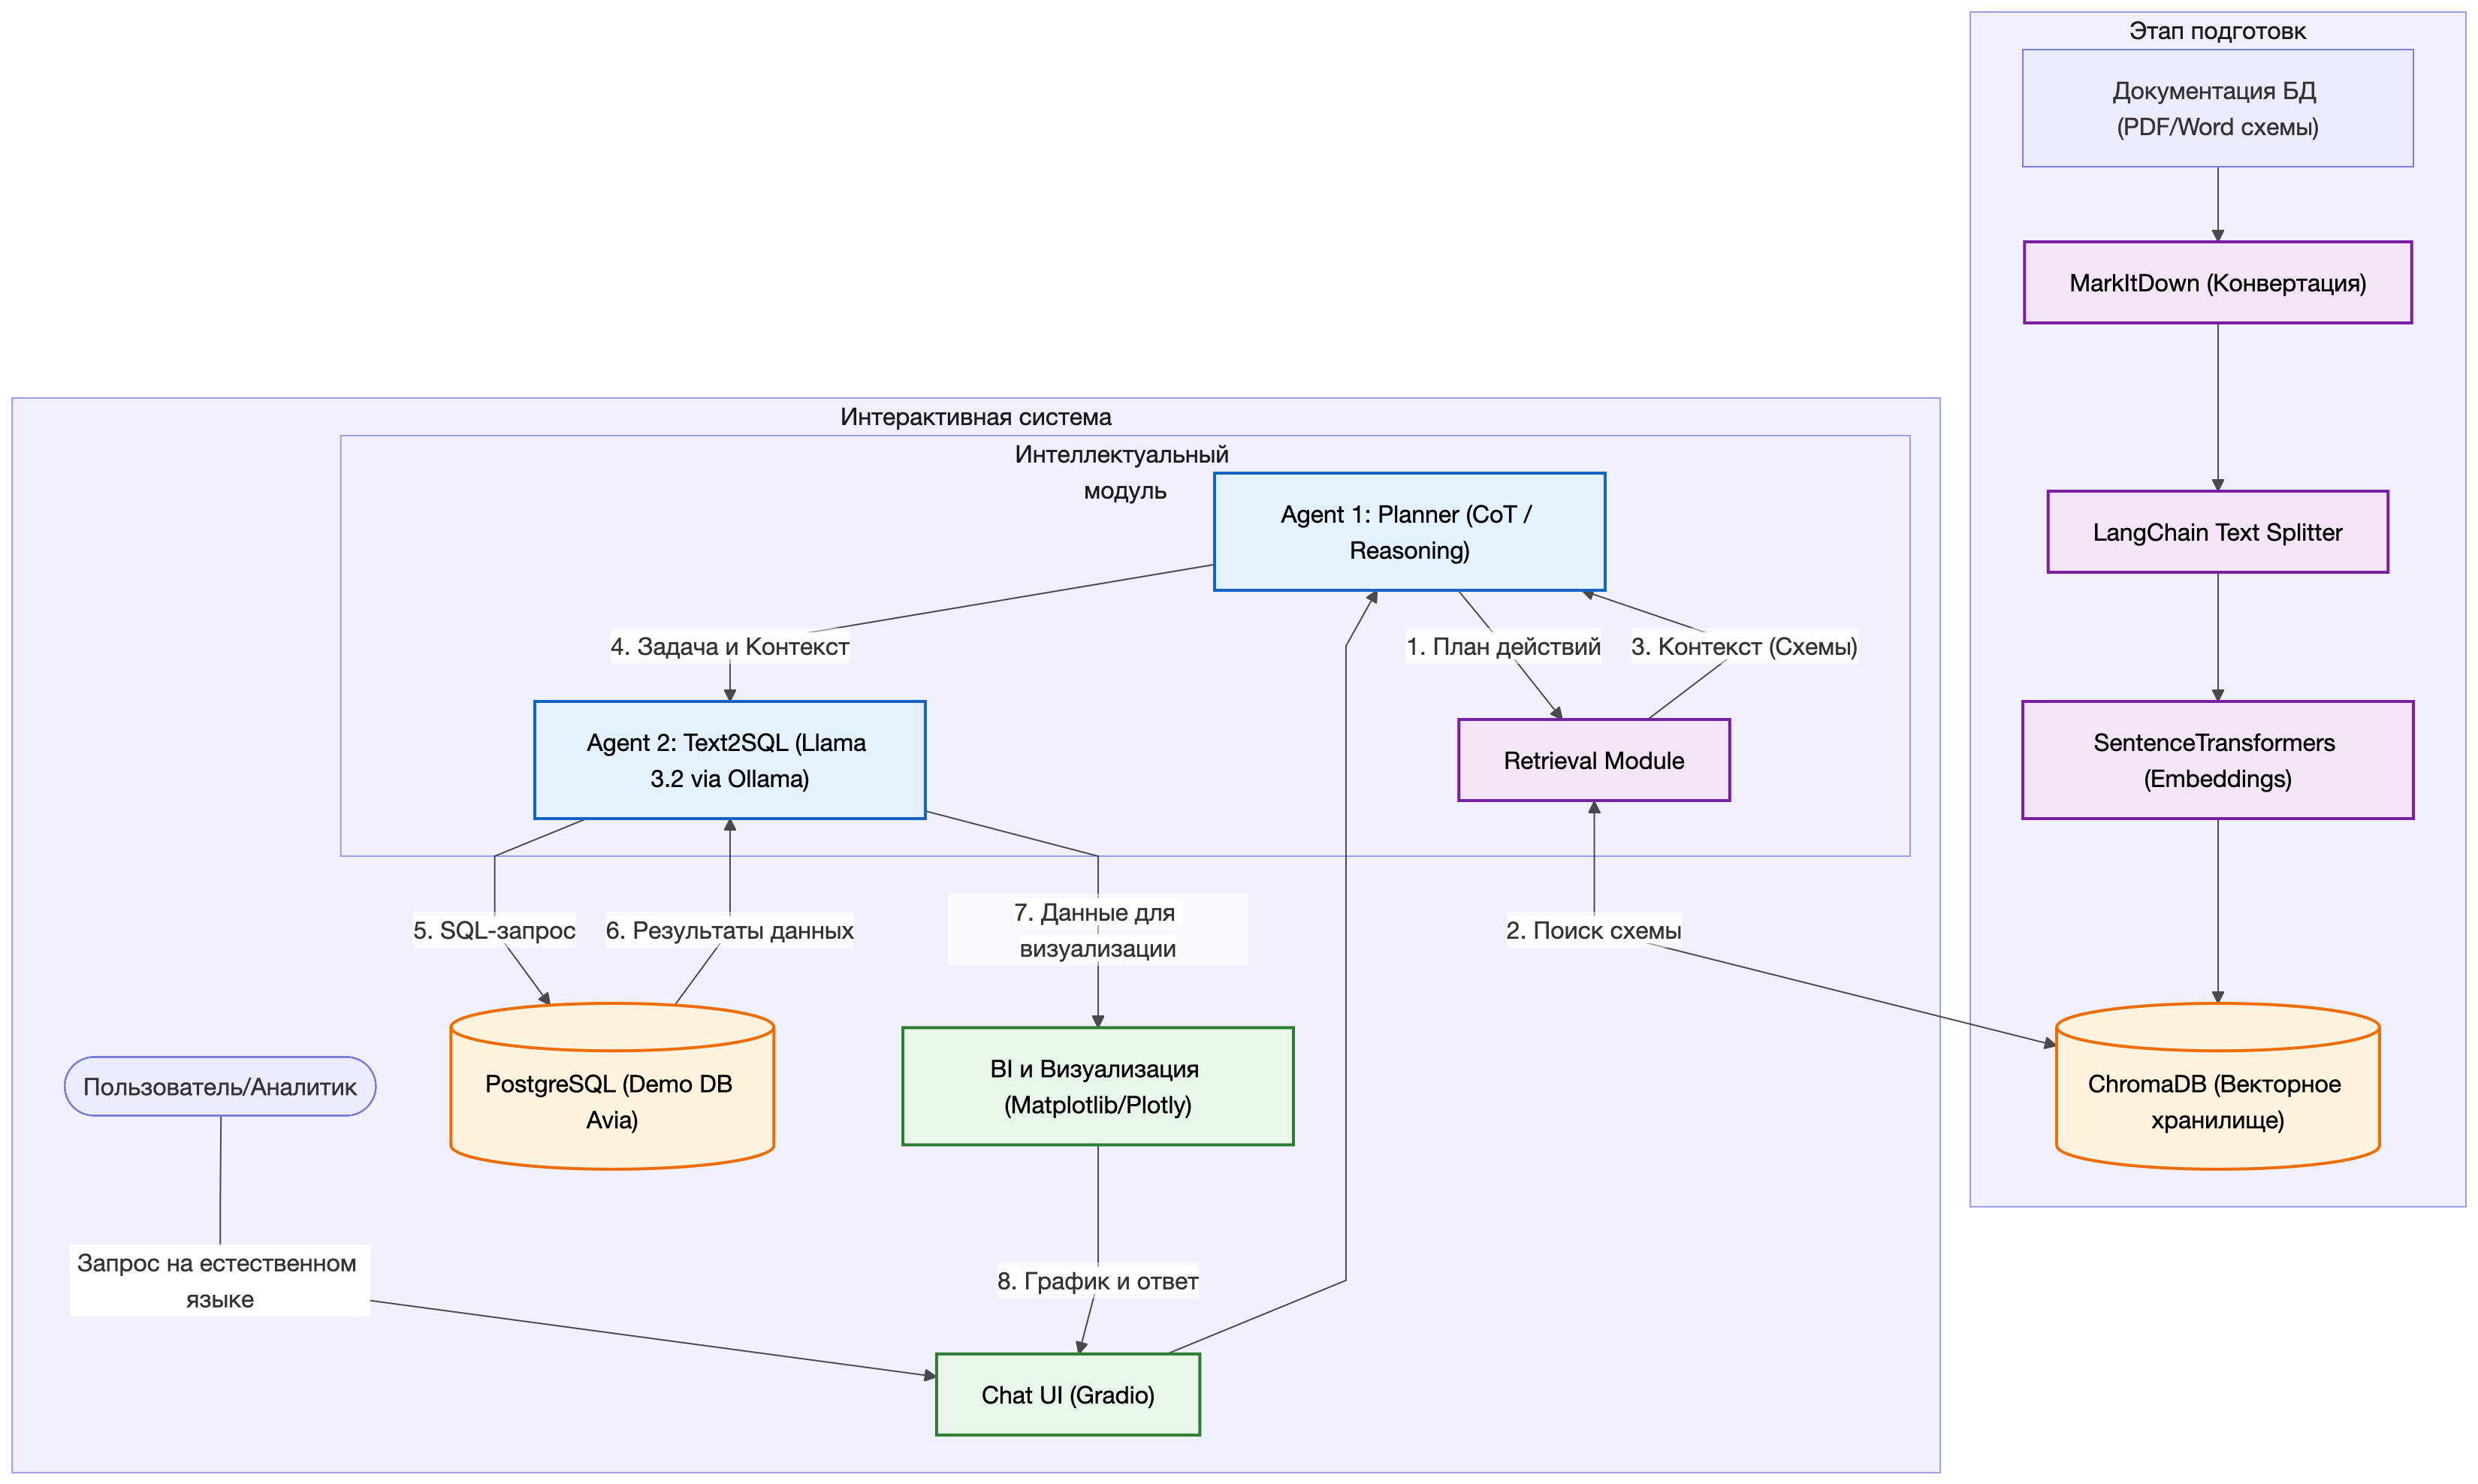
\includegraphics[width=0.75\textwidth]{./../materials/imgs/hld_system.png}
    
    \vspace{0.25cm} % Вертикальный отступ
    
    \textbf{Рис. 2:} Верхнеуровневая диаграмма 
\end{frame}

\begin{frame}{Flow}
    \centering % Центрирование изображения
    
    % Основная команда для вставки изображения
    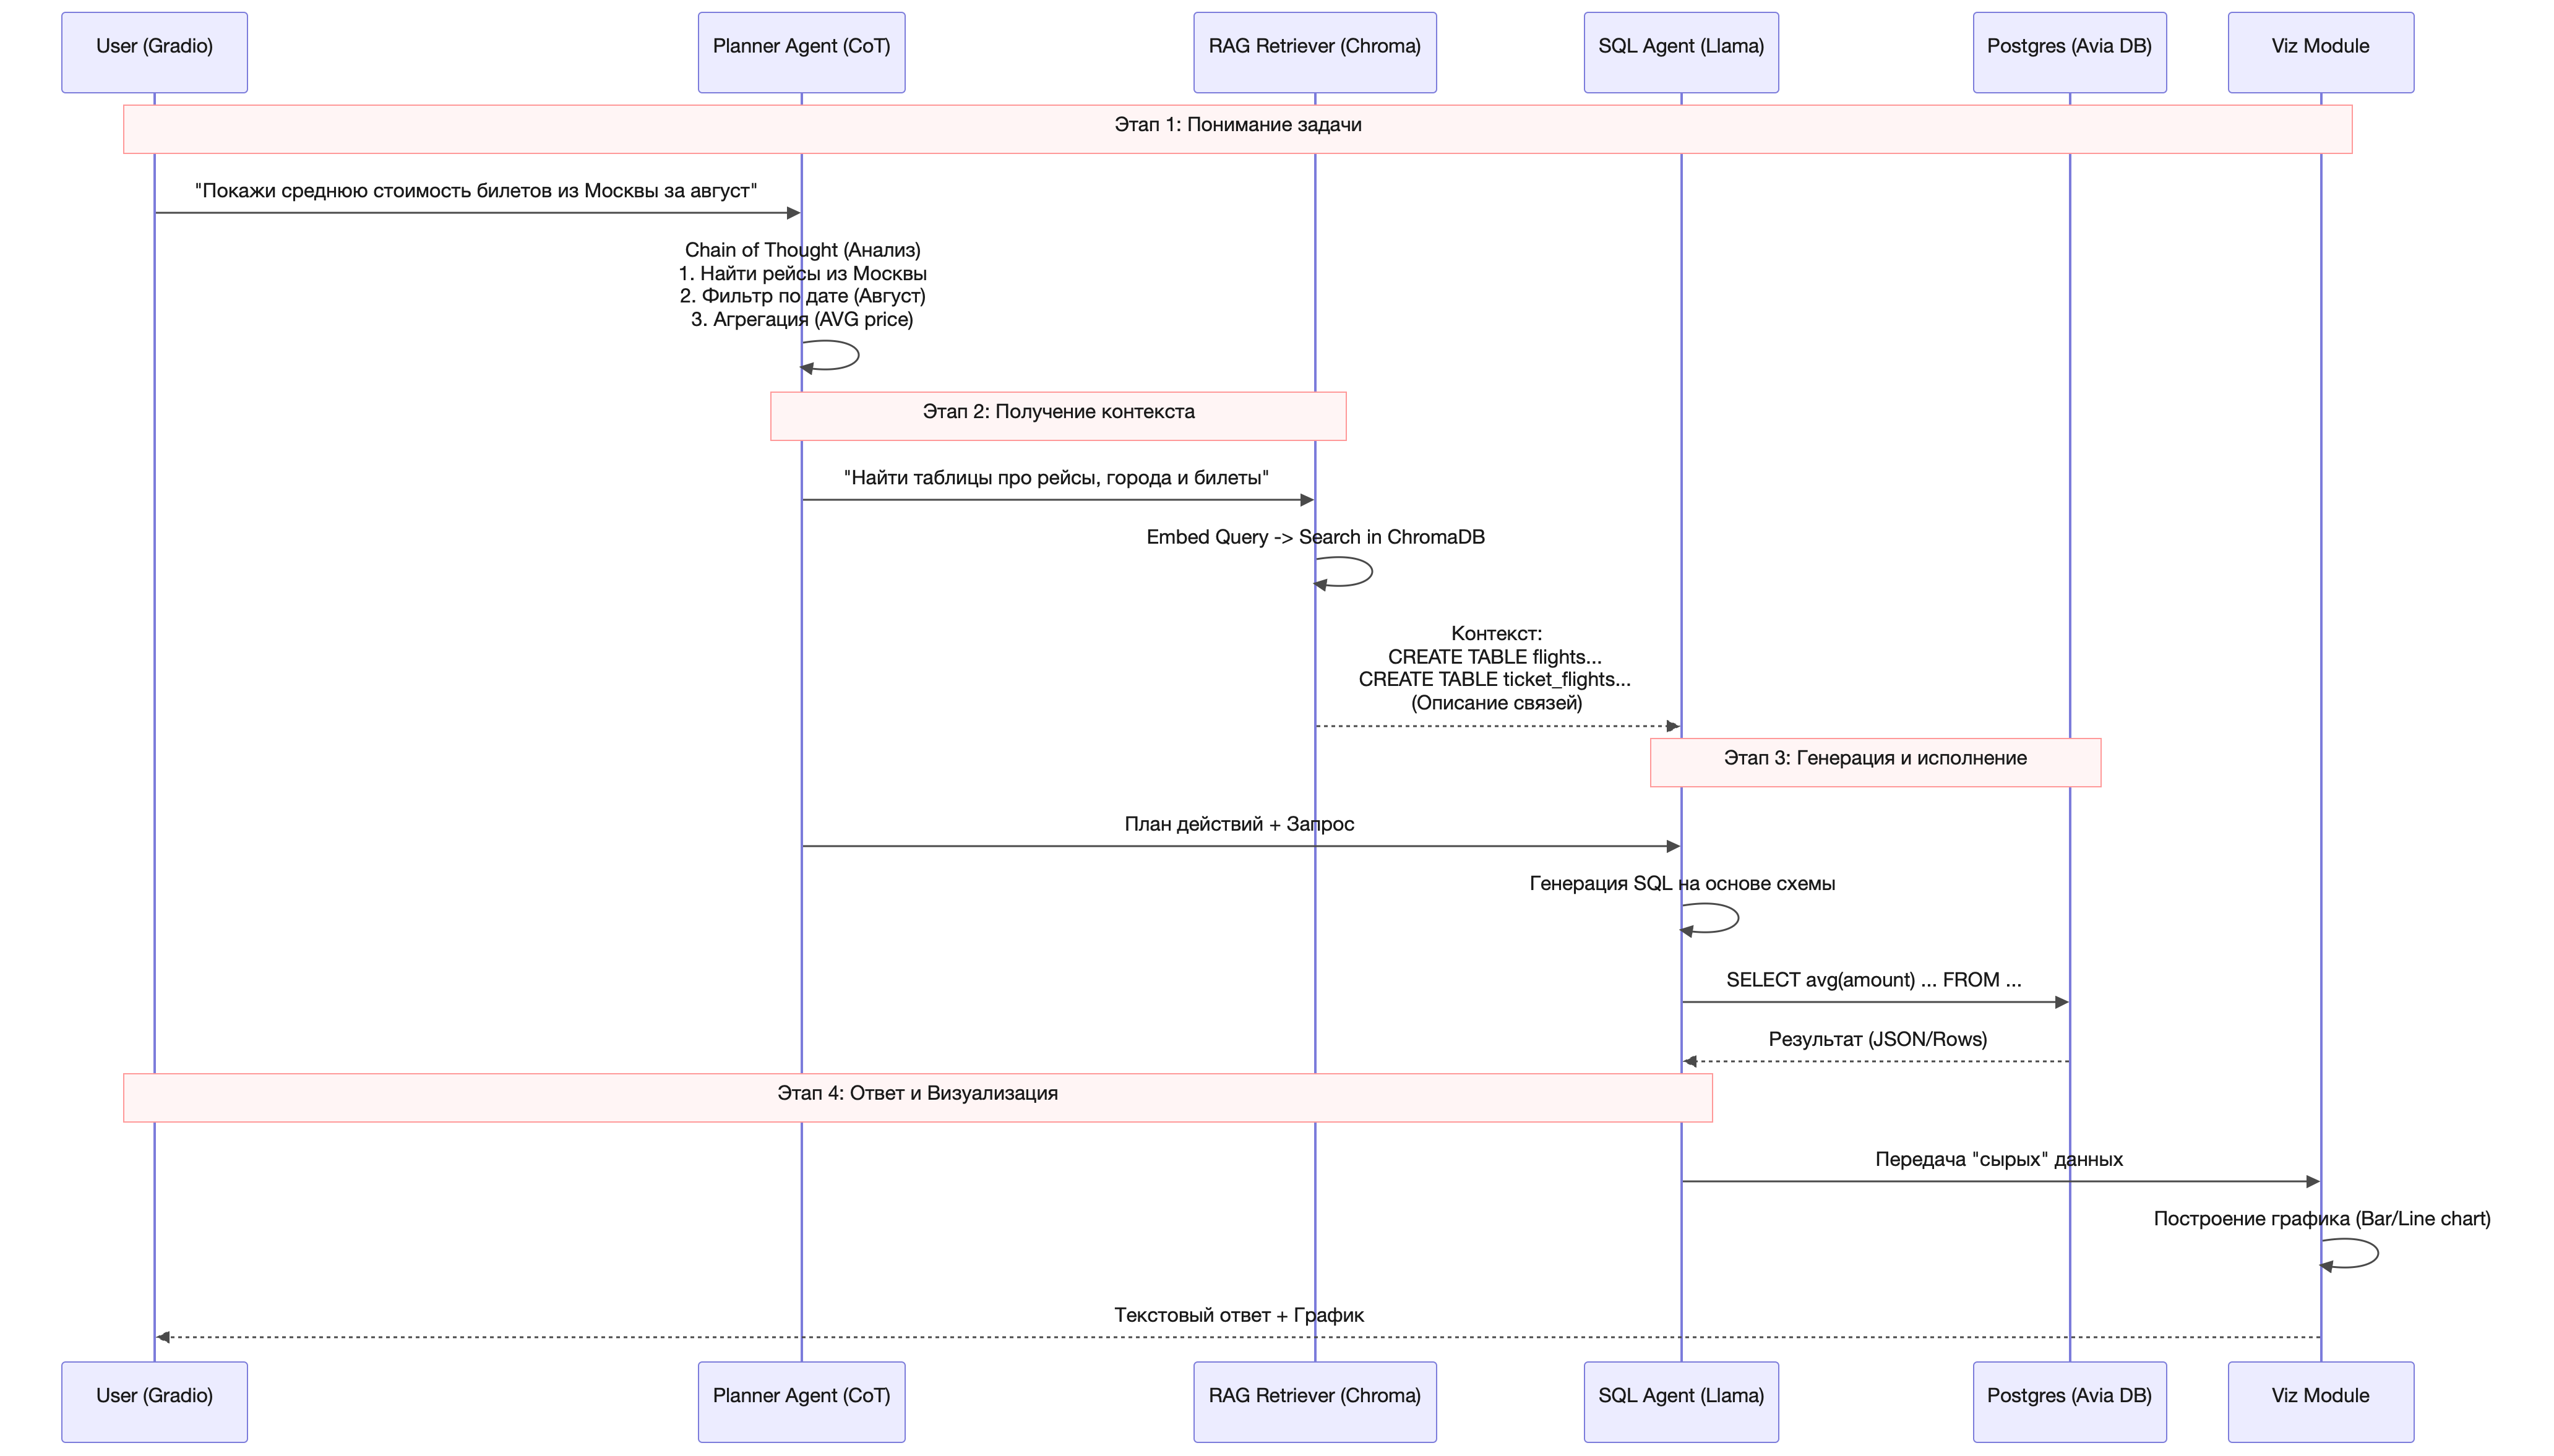
\includegraphics[width=0.75\textwidth]{./../materials/imgs/flow_chart.png}
    
    \vspace{0.25cm} % Вертикальный отступ
    
    \textbf{Рис. 3:} Pipeline использования 
\end{frame}



% ======================================================
% СЕКЦИЯ 5: Оставшиеся стадии
% ======================================================

\section{Дальнейшее развитие}

\begin{frame}{Дальнейшее развитие}
    Дальнейшие шаги развития проекта
    \begin{enumerate}
        \item Проэксперементировать с пайплайном RAG системы
        \item Добиться высокого показателя RAG системы при увеличении кол-ва таблиц в схеме
        \item Развертывание более большого дампа (за больший отчетный период)
        \item Довести все остальное до ума, доделать шаблон LaTeX и подготовить презентацию.
    \end{enumerate}
\end{frame}



% ======================================================
% СЕКЦИЯ 6: Концовка
% ======================================================

\section{Список использованных источников}

\begin{frame}{Список использованных источников}
    \footnotesize
    \begin{enumerate}
        % Книги и классика
        \item Дейт, К. Дж. Введение в системы баз данных / К. Дж. Дейт. — 8-е изд. — М. : Вильямс, 2016. — 1328 c.
        \item Рассел, С. Искусственный интеллект: современный подход / С. Рассел, П. Норвиг. — 3-е изд. — М. : Вильямс, 2019. — 1408 с.
        
        % Статьи по Text-to-SQL и RAG
        \item Lewis, P. Retrieval-Augmented Generation for Knowledge-Intensive NLP Tasks / P. Lewis, E. Perez et al. // Advances in Neural Information Processing Systems. — 2020. — Vol. 33. — P. 9459–9474.
        \item Zhong, V. Seq2SQL: Generating Structured Queries from Natural Language using Reinforcement Learning / V. Zhong, C. Xiong, R. Socher // arXiv preprint arXiv:1709.00103. — 2017.
        
        % Технологии и документация (как в вашем дипломе)
        \item Postgres Pro Standard : документация к СУБД. — 2024. — URL: https://postgrespro.ru/docs/ (дата обращения: 15.12.2024).
        \item LangChain Documentation : Retrieval-Augmented Generation (RAG). — 2024. — URL: https://python.langchain.com/docs/ (дата обращения: 06.11.2025).
        \item Ollama: Get up and running with large language models locally. — 2024. — URL: https://ollama.com/ (дата обращения: 20.12.2024).
        
        % Бенчмарки
        \item Yu, T. Spider: A Large-Scale Hierarchical Dataset for Semantic Parsing and Text-to-SQL Task / T. Yu, R. Zhang et al. // Proceedings of EMNLP. — 2018.
    \end{enumerate}
\end{frame}


\end{document}